In my 7th grade math class,\MarginComment{Ah the good old days of my youth...}
there was a clock that had on each hour label a different mathematical
expression that evaluated to that hour. For example, \( 8 \) wasn't just plain
old \( 8 \), but something like \( \sqrt{64} \) instead. I've always thought
this was a fun little recreational thing to nerd out about, but it slipped out
of my mind for the longest time.

I've since thought I should revisit this idea (mostly motivated by a bit of a
running joke that I'm having) and have a little fun crafting puzzles daily.
Compared to the clock though, they'll probably be a bit on the longer side (I
also anticipate that some problems will be easier to solve than make). Let's
get started!

\subsection{Problems}
\begin{enumerate}
    % % I'm trying to see if \filbreak is a good idea (probably wont put it for
    % the solutions because they get longer), so if this makes things wack,
    % just remove it I guess.
    % Ok yeah filbreak can break some stuff
    % \filbreak
    \item Let \( n \) be the order of the smallest possible subgroup of \( \left( \mathbb{R}, \cdot \right) \). Day \( n \).

    % \filbreak
    \item Day \( A \), where \( A \) represents the area of any triangle
        tangent to the curve \( y = 1 / x \) in the first quadrant and having
        vertices at the origin, \( x \)-axis, and \( y \)-axis.

    % \filbreak
    \item Let \( m \) be the \( 4 \)th digit of \( \tau \). Day \( m \). \MarginComment{The \( 4 \)th digit from the left, in case you needed clarification. ;)}

    % \filbreak
    \item Day
        \[
            2 \exp{\left( \frac{8}{\pi} \int_{ 0 }^{ 1 } \frac{\ln{\left( 1 + x \right)}}{x^2 + 1} \, dx \right)}
        .\]
        
    % \filbreak
    \item Day \( \abs{S_5} / \abs{S_4} \), where \( S_k \) denotes the
        symmetric group with degree \( k \).

    % \filbreak
    \item Let \( S \left( p \right) \) denote the number of times a permutation
        \( p \) must be composed until it reaches the identity permutation.
        Day \( S \left( \left( 1 \: 3 \right) \left( 2 \: 4 \: 5 \right) \right) \).

    % \filbreak
    \item Day \( D \), where \( D \) denotes the absolute distance between the
        eigenvalues of the following \( 2 \times 2 \) matrix:
        \[
            \begin{bmatrix}
                12099471394 & -8623006 \\
                121153998 & 12034827395
            \end{bmatrix}
        .\]

    % \filbreak
    \item Let \( N \) denote the number of distinct Fibonacci numbers that are perfect squares. Day \( 2^N \).

    % \filbreak
    \item Let \( \Gamma \) denote the unit circle, and define \( 13 \) circles
        \( \omega_0,\omega_1,\ldots,\omega_{12} \) such that they are all of
        equal radius \( r \) and externally tangent to \( \Gamma \). \MarginComment{I am
        definitely not the most experienced in Euclidean geometry so this might
        be a weird way to phrase the question.} In addition, each circle \(
        \omega_k \) is externally tangent to \( \omega_{(k - 1) \bmod{13}} \) and \( \omega_{(k
        + 1) \bmod{13}} \). Day \( \floor{30r} \).

    \item Big Boy Bill has a counter at value \( 0 \) and flips a fair, random
        coin \( 15 \) times. Every time he flips the coin, if it lands on
        heads, he adds \( 2 \) to the counter, and if it lands on tails, he
        adds \( 3 \) from the counter. There are \( m \) different sequences of
        coin flips in which at the end of the flipping, the resulting value is
        divisible by \( 5 \). Day \( 2m \bmod{23} \).
\end{enumerate}

\subsection{Solutions}
\begin{enumerate}
    \item By the definition of a group, it must at least include the identity
        element, meaning that the order must be positive. In general, the
        smallest and perhaps most trivial subgroup of a group is one containing
        solely the identity element (for this specific case the group is \(
        \left( \set{1}, \cdot \right) \)), thus our answer is \( \boxed{1} \).

        We shall give a general proof that the subgroup containing just the
        identity element exists.
        \begin{proof}
            We are given a group \( \left( G, \cdot \right) \) with identity
            \MarginComment{Ehh this feels a bit elementary but it's fine.}
            element \( e \). We shall prove that \( \left( \set{e}, \cdot
            \right) \) is a group and subsequently a subgroup of \( G \). We
            already have fulfilled the identity element condition required in
            the definition of a group, so all that is left is to verify that
            the inverse of \( e \) is in the subgroup (which would mean that it is equal to \( e \)).

            Suppose that \( e^{-1} = e \), giving us
            \[
                e \cdot e^{-1} = e^{-1} \cdot e = e \cdot e = e
            .\]
            This fulfills the condition to be an inverse, and thus \( \left(
            \set{e}, \cdot \right) \) is a group and a subgroup of \( G \).
        \end{proof}

    \item Let \( a \) be some positive real number. We shall find the line
        passing through \( \left( a, 1 / a \right) \) and tangent to the curve
        \( y = 1 / x \) to be
        \[
            y = 1 / a - 1 / a^2 \left( x - a \right)
        .\]
        Setting \( x \) and \( y \) to be zero individually and solving, we
        find that there is an \( x \)-intercept at \( \left( 2a, 0 \right) \)
        and a \( y \)-intercept at \( \left( 0, 2/a \right) \). This forms a right triangle
        with area \( 1 / 2 \cdot 2a \cdot 2 / a = \boxed{2} \).

    \begin{figure}[h]
        \centering
        \begin{tikzpicture}[domain=0.25:4, scale=1.2]
            \draw[<->, semithick] (-0.2, 0) -- (4.2, 0) node[right] {\small \( x \)};
            \draw[<->, semithick] (0, -0.2) -- (0, 4.2) node[above] {\small \( y \)};
            \draw[<->, thick, smooth] plot (\x, 1 / \x);

            \fill[fadegray!15, thick] (2, 0) -- (0, 2) -- (0, 0) -- cycle;
            \draw[fadegray, thick] (2, 0) -- (0, 2) -- (0, 0) -- cycle;

            \fill[fadegray] (1, 1) circle (1.5pt) node[above right] {\small \( \left( a, 1/a \right) \)};
            \fill[fadegray] (2, 0) circle (1pt) node[below] {\small \( \left( 2a, 0 \right) \)};
            \fill[fadegray] (0, 2) circle (1pt) node[left] {\small \( \left( 0, 2/a \right) \)};
        \end{tikzpicture}
        \caption{An example tangent triangle for Problem 2}
    \end{figure}
    
    \item Perhaps \MarginComment{I didn't put that much effort into making this
        problem as you can probably see.} you can figure this out with proper
        analytical methods, but \( \tau \approx 6.2832 \), so uhhhh... The
        answer is \( \boxed{3} \).

    \item We parametrize the inner integral as such:
        \[
            I \left( a \right) = \int_{ 0 }^{ 1 } \frac{\ln{\left( 1 + ax \right)}}{x^2 + 1} \, dx
        ,\]
        giving us an initial condition that \( I \left( 0 \right) = 0 \). We
        can then differentiate both sides with respect to \( a \) and do some
        integrating:
        \begin{align*}
            I' \left( a \right) &= \int_{ 0 }^{ 1 } \frac{x}{( 1 + ax ) ( x^2 + 1 )} \, dx \\
            &= \frac{1}{a^2 + 1} \int_{ 0 }^{ 1 } \frac{x + a}{x^2 + 1} \, dx - \frac{a}{a^2 + 1} \int_{ 0 }^{ 1 } \frac{1}{ax + 1} \, dx \\
            &= \bounds{\frac{1}{2 ( 1 + a^2 )} \ln{\abs{x^2 + 1}}}{0}{1} + \bounds{\frac{a}{a^2 + 1} \arctan{x}}{0}{1} - \bounds{\frac{1}{a^2 + 1} \ln{\abs{1 + ax}}}{0}{1} \\
            &= \frac{\ln{2}}{2 (1 + a^2)} + \frac{\pi a}{4 (1 + a^2)} - \frac{\ln{\left( 1 + a \right)}}{a^2 + 1}
        .\end{align*}
        Now we can solve for \( I \left( 1 \right) \), which is exactly our
        desired integral. \MarginComment{Yes that is tau you see in the
        integral bounds. Tau for tau day.}
        \begin{align*}
            I \left( 1 \right) &= I \left( 0 \right) + \int_{ 0 }^{ 1 } I' \left( \tau \right) \, d\tau \\
            &= \frac{\pi \ln{2}}{8} + \frac{\pi \ln{2}}{8} - \int_{ 0 }^{ 1 } \frac{\ln{\left( \tau + 1 \right)}}{\tau^2 + 1} \, d\tau \\
            &= 2 \cdot \frac{\pi \ln{2}}{8} - I \left( 1 \right) \\
            \implies I \left( 1 \right) &= \frac{\pi \ln{2}}{8}
        .\end{align*}
        Now we can plug this in and simplify the given expression:
        \begin{align*}
            &2 \exp{\left( \frac{8}{\pi} \int_{ 0 }^{ 1 } \frac{\ln{\left( 1 + x \right)}}{x^2 + 1} \, dx \right)} \\
            &= 2 \exp{\left( \frac{8}{\pi} \cdot \frac{\pi \ln{2}}{8} \right)} \\
            &= 2 \exp{\left( \ln{2} \right)} \\
            &= \boxed{4}
        .\end{align*}

    \item The order of the symmetric group \( S_k \) is simply \( k! \), so the answer is \( 5!/4! = \boxed{5} \).

    \item One can either manually multiply the permutation out until it reaches
        the identity permutation or realize that because it is factored into
        two disjoint cycles of length \( 2 \) and \( 3 \), it will require \(
        \gcd{\left( 2, 3 \right)} = \boxed{6} \) compositions to return to the identity
        permutation.

    \item The eigenvalues of the matrix are given by the solutions to the following polynomial:
        \[
            \left( \lambda - 12099471394 \right) \left( \lambda - 12034827395 \right) + 8623006 \cdot 121153998 = 0
        .\]
        Notice that distance between the roots is exactly the discriminant, which is
        \begin{align*}
            D &= \sqrt{\left( 12099471394 + 12034827395 \right)^2 - 4 \left( 12099471394 \cdot 12034827395 + 8623006 \cdot 121153998 \right)} \\
            &= \boxed{7}
        .\end{align*}

    \item It has been proven \MarginComment{While I would have liked to give a
        proof of this statement it turns out to involve a bit of machinery.}
        that the only three perfect square Fibonacci numbers are \( 0, 1\), and
        \( 144 \). Thus, our answer is \( 2^3 = \boxed{8} \).

    \item This one took me a bit and a half to compose. \MarginComment{Future
        Rushil here. Hahahahaha I overcomplicated this solution a lot. If you
        consider a 13-gon with radius \( 1 + r \) and then find the distance
        between the vertices with some light trig, everything pops out quite well (credit
        to Kelly for that :skull:).} Essentially what I'm trying to convey is
        that the each circle \( \omega_k \) is tangent to the previous and next
        circle and the center unit circle, forming a ring of circles.

    \begin{figure}
        \begin{minipage}{0.5\textwidth}
            \centering
            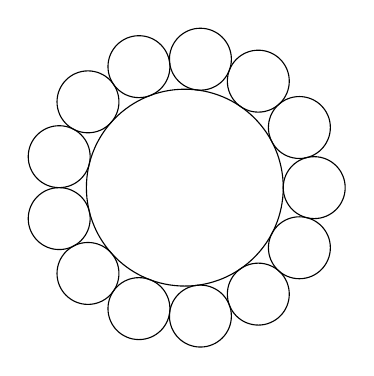
\begin{tikzpicture}[scale=1.25]
                \draw (0, 0) circle (1);

                \foreach \k in {0,...,12} {
                    \draw ({1.3146 * cos(360 * \k / 13)}, {1.3146 * sin(360 * \k / 13)}) circle (0.3146);
                }
            \end{tikzpicture}
            \caption{The idea Problem 9 is trying to convey.}
        \end{minipage}
        \begin{minipage}{0.5\textwidth}
            \centering
            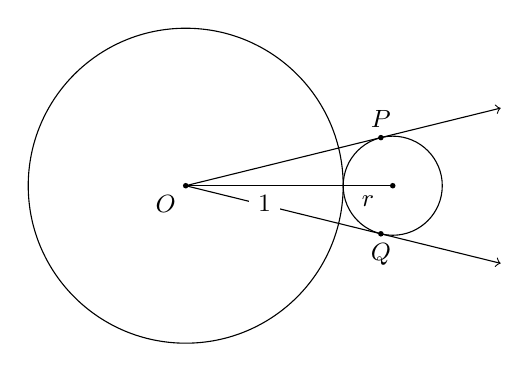
\begin{tikzpicture}[scale=2]
                \draw (0, 0) circle (1);
                \fill (0, 0) circle (0.5pt) node[below left] {\small \( O \)};

                \draw (1 + 0.3146, 0) circle (0.3146);
                \fill (1 + 0.3146, 0) circle (0.5pt);

                \draw[->] (0, 0) -- (2, {2 * 0.3146 / sqrt(2 * 0.3146 + 1)});
                \draw[->] (0, 0) -- (2, {-2 * 0.3146 / sqrt(2 * 0.3146 + 1)});
                \fill ({2 - 1 / (0.3146 + 1)}, {0.3146 / sqrt(2 * 0.3146 + 1) * (2 - 1 / (0.3146 + 1))}) circle (0.5pt) node[above] {\small \( P \)};
                \fill ({2 - 1 / (0.3146 + 1)}, {-0.3146 / sqrt(2 * 0.3146 + 1) * (2 - 1 / (0.3146 + 1))}) circle (0.5pt) node [below] {\small \( Q \)};

                \draw (0, 0) -- (1, 0) node[midway, below, fill=white] {\small \( 1 \)};
                % \node[below] at (0.5, 0) {}
                \draw (1, 0) -- (1 + 0.3146, 0) node[midway, below] {\small \( r \)};
            \end{tikzpicture}
            \caption{A diagram for the solution to Problem 9.}
        \end{minipage}
    \end{figure}

    Construct a circle, we'll call this \( \omega_0 \) of some unknown radius
    \( r \) that is externally tangent to \( \Gamma \). For simplicity, we'll
    pull it to the exact right of \( \Gamma \). Let \( O \) be the center of \(
    \Gamma \) and \( P,Q \) respectively be the points lying on the two tangent
    lines to \( \omega_0 \) extending from \( O \). Notice that \( 2 \pi /
    \angle POQ \) should be the number of circles that one can fit around \(
    \Gamma \), in other words, \( 13 \).

    Notice that if we find the slope \( a \) of \( \overrightarrow{OP} \), we
    can find \( \angle POQ = 2 \arctan{a} \). This motivates us to use analytic
    methods \MarginComment{There might be a more "geometric" solution, but this
    is the method that I used.}. 

    If we take \( O \) to be the origin, we can represent \( \omega_0 \) by
    \[
        \left( x - \left( 1 + r \right) \right)^2 + y^2 = r^2
    ,\]
    and we can let \( \overrightarrow{OP} \) be represented by the line \( y =
    ax \). If we substitute this expression for \( y \) into the equation for
    \( \omega_0 \) and set the discriminant equal to \( 0 \) (because this line
    is tangent to \( \omega_0 \)), we can obtain an expression for \( a \) in
    terms of \( r \) as follows:
    \begin{align*}
        \omega_0 \colon 0 &= \left( a^2 + 1 \right) x^2 - 2 \left( 1 + r \right)x + \left( 1 + r \right)^2 - r^2 \\
        \implies 0 &= 4 \left( 1 + r \right)^2 - 4 \left( a^2 + 1 \right) \left( 2r + 1 \right) \\
        a &= \frac{r}{\sqrt{2r + 1}}
    .\end{align*}
    We can now substitute this into our condition of \( 13 \) circles to get
    \begin{align*}
        \frac{2 \pi}{\angle POQ} &= 13 \\
        \implies \frac{\pi}{\arctan{a}} &= 13 \\
        \implies \frac{r}{\sqrt{2r + 1}} &= \tan{\left( \frac{\pi}{13} \right)}
    .\end{align*}
    Solving this for the positive root gives us \( r \approx 0.3146 \), which means that \( \floor{30r} = \boxed{9} \).

    \item Suppose BBB \MarginComment{BBB is the shorthand for Big Boy Bill, for
        those unaware.} flips \( k \) heads. Necessarily, this means he must
        have flipped \( 15 - k \) tails. From this, we can calculate the ending
        counter value and then take it modulo \( 5 \) to find the values of \(
        k \) that make our condition hold. Doing so, we can see that
        \begin{align*}
            2k + 3 \left( 15 - k \right) &\equiv 0 \pmod{5} \\
            \implies k &\equiv 0 \pmod{5}
        .\end{align*}
        As such, the only legal values of \( k \) that make the counter value
        divisible by \( 5 \) are \( 0, 5, 10 \), and \( 15 \). We're now
        looking for sequences of flips where we \textit{choose} \( 0, 5, 10 \),
        or \( 15 \) heads, which we can count to be
        \[
            \binom{15}{0} + \binom{15}{5} + \binom{15}{10} + \binom{15}{15} = 6008
        .\]
        Now all that's left is to see that \( 2 \cdot 6008 \bmod{23} = \boxed{10} \).

\end{enumerate}
